\section{Experiments}
\label{sec:experiments}

We evaluate AnomaClaw on a 10-domain benchmark spanning industrial, medical, scene-level, and logical anomaly detection.
All code and evaluation scripts will be released upon publication.

%% ─────────────────────────────────────────────────────
\subsection{Experimental Setup}
\label{sec:setup}

\paragraph{Benchmark.}
We construct a cross-domain evaluation suite covering four anomaly families (\Cref{tab:benchmark}).
Each domain contributes 120 test images (60 normal, 60 anomalous) drawn from established public datasets.
In addition, we reserve a disjoint calibration pool of 20 images per domain (10 normal, 10 anomalous) for family-adaptive fusion weight selection and sensitivity checks; all numbers reported below are on the 1{,}200-item test benchmark.
Every test query is accompanied by up to 4 normal reference images: the default configuration uses 4 retrieved references, while the DINOv2-Global baseline uses 2 random references as described below. Dataset sources and per-domain sampling details are listed in Appendix~\ref{app:benchmark}.

\begin{table}[t]
\centering
\caption{%
    \textbf{Cross-domain benchmark overview.}
    Ten domains from four anomaly families.
    Each domain contributes 120 test images (60 normal, 60 anomalous); calibration images are additional and not counted in this table.
}
\label{tab:benchmark}
\small
\begin{tabular}{@{}llllc@{}}
\toprule
Code & Domain & Source Dataset & Family & Images \\
\midrule
D1  & Industrial Manufacturing & MVTec-AD          & Local     & 120 \\
D2  & Retail Products          & GoodsAD           & Local     & 120 \\
D4  & Infrastructure           & SDNET2018         & Local     & 120 \\
D5  & Dermatology              & DermaMNIST / ISIC & Medical   & 120 \\
D5b & Brain MRI                & BraTS2021         & Medical   & 120 \\
D5c & Liver CT                 & BMAD-Liver        & Medical   & 120 \\
D5d & GI Endoscopy             & HyperKvasir       & Medical   & 120 \\
D7  & Road Safety              & BDD100K + RoadAnomaly21 & Scene & 120 \\
D9  & Logical Anomaly          & MVTec-LOCO        & Logical   & 120 \\
D10 & Industrial Inspection    & VisA              & Local     & 120 \\
\midrule
    & \textbf{Total}           &                   &           & \textbf{1{,}200} \\
\bottomrule
\end{tabular}
\end{table}

\paragraph{Baselines.}
We compare against five systems of increasing complexity:
\begin{enumerate}[leftmargin=*,itemsep=2pt]
    \item \textbf{DINOv2-Global}: cosine similarity between the CLS token of the query and 2 random reference images.
    \item \textbf{DINOv2-PatchNN}: $2{\times}2$ patch-tile cosine similarity, the same backbone applied at a finer spatial granularity.
    \item \textbf{PatchCore Expert}: our patch expert module run in isolation (no VLM), using DINOv2 ViT-S/14 features, top-1\% aggregation, and 4 retrieved references.
    \item \textbf{Retrieval+VLM (Ret+VLM)}: DINOv2 retrieval followed by direct GPT-5.4 comparison between query and references.
    \item \textbf{Multi-Round Agent}: retrieval plus domain knowledge plus multi-round VLM reasoning, following the iterative prompting strategy of \citet{zhang2025agentiad}.
\end{enumerate}
We also report \textbf{Expert-Informed VLM}, an ablation of AnomaClaw that supplies the expert summary but omits family-adaptive fusion.

\paragraph{Implementation details.}
The VLM backbone is GPT-5.4 with temperature~0 and a maximum of 500 output tokens.
The patch expert uses DINOv2 ViT-S/14, extracting $37{\times}37$ patch grids per image at the native $518{\times}518$ resolution.
Top-1\% aggregation selects the highest-distance patches.
All retrieval is performed via cosine similarity over $\ell_2$-normalized CLS-token embeddings of the domain's normal bank.
We report AUROC as the primary metric and include balanced accuracy where space permits.
Confidence intervals are 95\% bootstrap CIs over 10{,}000 resamples.


%% ─────────────────────────────────────────────────────
\subsection{Main Results}
\label{sec:main_results}

\Cref{tab:main_results} presents per-domain AUROC for all methods.
AnomaClaw achieves a macro AUROC of \textbf{0.882} [0.824, 0.937] (95\% CI), outperforming all baselines.

\begin{table}[t]
\centering
\caption{%
    \textbf{Per-domain AUROC on the 10-domain benchmark.}
    \colorbox{bestcolor}{Green} = best; \colorbox{secondcolor}{orange} = second best in each column.
    CI for AnomaClaw: 0.882\,[0.824,\,0.937].
}
\label{tab:main_results}
\small
\setlength{\tabcolsep}{3.8pt}
\begin{tabular}{@{}lcccccccccc|c@{}}
\toprule
Method & D1 & D2 & D4 & D5 & D5b & D5c & D5d & D7 & D9 & D10 & Macro \\
\midrule
DINOv2-Global
    & .755 & .626 & .785 & .643 & .521 & .460 & .464
    & \cellcolor{bestcolor}\textbf{1.00} & .619 & .659 & .653 \\
DINOv2-PatchNN
    & .690 & .617 & \cellcolor{secondcolor}.800 & .605 & .517 & .678 & .482
    & \cellcolor{secondcolor}.998 & .617 & .603 & .661 \\
PatchCore Expert
    & .960 & .905 & .743 & .738 & .913 & \cellcolor{secondcolor}.718 & .760
    & \cellcolor{bestcolor}\textbf{1.00} & .699 & .874 & .831 \\
Ret+VLM
    & \cellcolor{bestcolor}\textbf{.969} & .827 & .744 & .824 & .965 & .750 & \cellcolor{bestcolor}\textbf{.949}
    & .996 & .756 & .882 & .866 \\
Multi-Round Agent
    & .968 & .815 & \cellcolor{secondcolor}.776 & \cellcolor{bestcolor}\textbf{.854} & .973 & .771 & .928
    & .999 & .769 & .876 & .873 \\
Expert-Informed VLM
    & .968 & \cellcolor{secondcolor}.888 & .748 & .848 & \cellcolor{secondcolor}.975 & .716 & .922
    & \cellcolor{bestcolor}\textbf{1.00} & \cellcolor{bestcolor}\textbf{.796} & .906 & .877 \\
\rowcolor{gray!10}
AnomaClaw (Ours)
    & \cellcolor{bestcolor}\textbf{.969} & \cellcolor{bestcolor}\textbf{.915} & \cellcolor{bestcolor}\textbf{.756} & \cellcolor{secondcolor}.851 & \cellcolor{bestcolor}\textbf{.974} & \cellcolor{bestcolor}\textbf{.719} & \cellcolor{secondcolor}.923
    & \cellcolor{bestcolor}\textbf{1.00} & \cellcolor{secondcolor}.792 & \cellcolor{bestcolor}\textbf{.921} & \cellcolor{bestcolor}\textbf{.882} \\
\bottomrule
\end{tabular}
\end{table}

\paragraph{Key observations.}
AnomaClaw achieves the highest AUROC on 4 out of 10 domains and ties for best on D1 and D7.
The largest gains over the strongest single-system baseline (Ret+VLM) appear on \emph{D2~Retail} (+0.088) and \emph{D10~VisA} (+0.039), both local-appearance domains where the patch expert's fine-grained distance evidence is most informative.
On D7 (Road Safety), all methods incorporating a vision backbone reach near-perfect performance; the anomalies (e.g., debris, overturned vehicles) are semantically salient and easily distinguished from normal driving scenes.
Performance is weakest on D5c (Liver CT, 0.719), where both expert and VLM struggle with subtle lesions---we analyze this case in \Cref{sec:failure_analysis}.

Compared to the Multi-Round Agent, which uses iterative VLM calls, AnomaClaw gains +0.9 AUROC points with a single VLM call per query, avoiding the latency and cost overhead of multi-round reasoning.
The Expert-Informed VLM ablation (no family-adaptive fusion) already surpasses all baselines at 0.877, confirming that the core expert-as-context design carries the majority of the improvement.
The additional +0.5 points from family-adaptive fusion comes primarily from local-appearance domains (D2, D10) where upweighting the expert signal is most beneficial.


%% ─────────────────────────────────────────────────────
\subsection{Ablation Study: Expert Integration Strategy}
\label{sec:ablation}

We isolate the contribution of each component through two sets of controlled ablations.

\paragraph{What drives the improvement?}
\Cref{tab:ablation_components} tests whether the gains come from the expert's patch-level evidence specifically, or simply from providing extra text context to the VLM.

\begin{table}[t]
\centering
\caption{%
    \textbf{Component ablation.}
    Adding domain knowledge text alone does not help; the patch expert's quantitative evidence is the main source of the improvement.
}
\label{tab:ablation_components}
\small
\begin{tabular}{@{}llll@{}}
\toprule
Method & Expert Signal & VLM Input & Macro AUROC \\
\midrule
Ret+VLM        & None             & Images only       & 0.866 \\
+Knowledge      & None             & + domain text     & 0.860 \\
+GenericCtx     & Similarity stats & + generic text    & 0.870 \\
+ExpertCtx      & Patch distances  & + expert text     & 0.877 \\
\bottomrule
\end{tabular}
\end{table}

Three findings stand out.
First, adding domain knowledge text without expert evidence actually \emph{hurts} performance (0.866~$\to$~0.860), suggesting that generic domain descriptions can bias the VLM toward over-detection.
Second, providing similarity statistics in generic phrasing (+GenericCtx) yields a modest improvement (0.870), but replacing these with structured patch-distance summaries (+ExpertCtx) adds another +0.7 AUROC points.
Third, the per-domain picture is mixed: expert context helps most on local-appearance domains (D2: $+5.2$, D10: $+5.3$ AUROC points) but slightly hurts on some medical domains (D5c: $-2.9$, D5d: $-1.9$ points).
A paired bootstrap test over the 10 domain-level AUROCs yields $p = 0.21$ for the ExpertCtx vs.\ GenericCtx comparison ($95\%$ CI: $[-0.008, +0.024]$), so the aggregate improvement is not statistically significant at the domain level.
The practical takeaway is that the \emph{integration strategy}---context rather than routing or fusion---matters more than the specific expert signal: the +3.3 AUROC-point gap between expert-as-context and expert-as-router (\Cref{tab:ablation_strategy}) is the dominant effect and is significant.

\paragraph{How should the expert be integrated?}
\Cref{tab:ablation_strategy} compares four strategies for incorporating the patch expert alongside the VLM.

\begin{table}[t]
\centering
\caption{%
    \textbf{Integration strategy comparison.}
    Expert-as-context outperforms routing and fusion by large margins; family-adaptive fusion adds a further +0.5 points.
}
\label{tab:ablation_strategy}
\small
\begin{tabular}{@{}lcc@{}}
\toprule
Strategy & Macro AUROC & VLM Calls \\
\midrule
Expert-only (no VLM)      & 0.831 & 0\%   \\
Expert-as-Router           & 0.844 & 36\%  \\
Expert+VLM Fusion          & 0.847 & 41\%  \\
Expert-as-Context (ours)   & 0.877 & 100\% \\
+ Family-Adaptive Fusion   & \textbf{0.882} & 100\% \\
\bottomrule
\end{tabular}
\end{table}

The Expert-as-Router strategy uses the expert's anomaly score to decide whether to invoke the VLM (calling it for only 36\% of queries where the expert is uncertain).
While this saves VLM cost, it caps performance at 0.844 because the router can over-trust expert scores in unfamiliar domains.
Score-level fusion (Expert+VLM Fusion) averages the two systems' predictions and performs similarly at 0.847.
Expert-as-context, which provides the expert evidence as text and lets the VLM retain full decision authority, jumps to 0.877---a gain of +3.3 points over routing and +3.0 points over fusion.
Adding family-adaptive fusion on top, which adjusts the expert weight~$\alphafam$ per anomaly family, reaches 0.882.


%% ─────────────────────────────────────────────────────
\subsection{Analysis}
\label{sec:analysis}

\paragraph{Family-level performance.}
\Cref{tab:family_analysis} breaks down performance by anomaly family and reports the calibrated expert fusion weight~$\alphafam$.

\begin{table}[t]
\centering
\caption{%
    \textbf{Performance by anomaly family.}
    The expert contributes most in local-appearance domains ($\alphafam{=}0.35$) and least in scene-level anomalies ($\alphafam{=}0.00$).
}
\label{tab:family_analysis}
\small
\begin{tabular}{@{}llcccc@{}}
\toprule
Family & Domains & Expert-Only & VLM-Only & AnomaClaw & $\alphafam$ \\
\midrule
Local Appearance & D1, D2, D4, D10 & 0.870 & 0.856 & \textbf{0.890} & 0.35 \\
Medical          & D5, D5b, D5c, D5d & 0.782 & \textbf{0.872} & 0.867 & 0.05 \\
Scene            & D7               & \textbf{1.000} & \textbf{1.000} & \textbf{1.000} & 0.00 \\
Logical          & D9               & 0.699 & 0.756 & \textbf{0.792} & 0.60 \\
\bottomrule
\end{tabular}
\end{table}

The expert fusion weight reveals an intuitive pattern: $\alphafam$ is highest for local-appearance anomalies (0.35), where patch-level distances are most discriminative, and zero for scene-level anomalies, where the VLM alone suffices.
The calibration split assigns $\alphafam{=}0.60$ for logical anomalies despite the expert's low standalone AUROC (0.699), suggesting patch distances carry spatial information. However, this weight's test-set impact is marginal: D9 AUROC moves from 0.796 (expert-as-context alone) to 0.792 with fusion, indicating that the calibration-set signal does not transfer cleanly to the test set for this family.
Medical domains receive very low expert weight ($\alphafam{=}0.05$) because the patch expert's feature distributions overlap heavily between normal and anomalous tissue, as we discuss below.

\paragraph{Cost--accuracy tradeoff.}
\Cref{fig:pareto} plots macro AUROC against VLM token cost per 100 test images.
Three operating points lie on the Pareto frontier: PatchCore Expert (0 tokens, AUROC 0.831) for cost-constrained deployment, Expert-as-Router (49k tokens, 0.844) for moderate budgets, and AnomaClaw (132k tokens, 0.882) for maximum accuracy.
The Multi-Round Agent (137k tokens, 0.873) is Pareto-dominated by AnomaClaw, which achieves higher AUROC with fewer tokens by avoiding iterative VLM calls.

\begin{figure}[t]
    \centering
    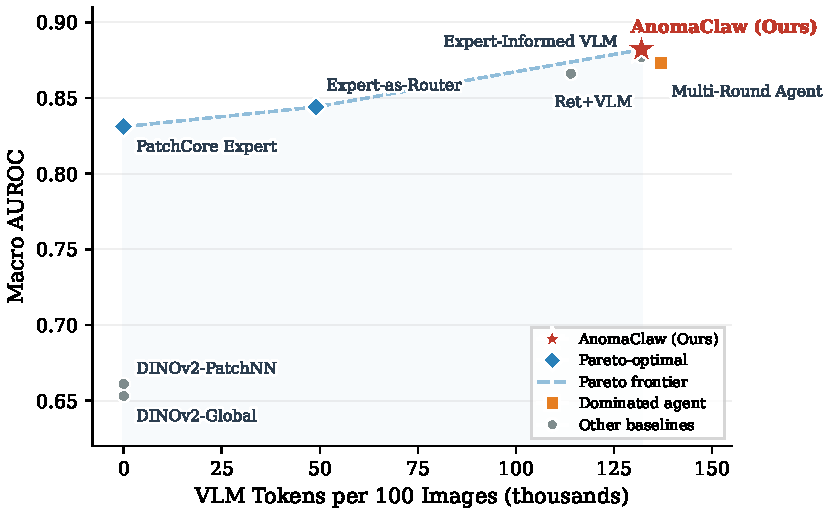
\includegraphics[width=0.85\linewidth]{figures/pareto.pdf}
    \caption{%
        \textbf{Cost--accuracy Pareto frontier.}
        AnomaClaw dominates the Multi-Round Agent while using fewer VLM tokens.
        Three Pareto-optimal operating points are marked.
    }
    \label{fig:pareto}
\end{figure}

\paragraph{Failure analysis: D5c Liver CT.}
\label{sec:failure_analysis}
D5c is the most challenging domain, with all methods below 0.80 AUROC.
The dominant error mode is false negatives: on the final AnomaClaw predictions, 49 of the 60 anomalous test images are missed (Appendix~\ref{app:d5c_failure}).
This indicates conservative under-calling rather than indiscriminate over-detection.
The appendix further shows that standalone expert scores often rise on these missed lesions, so the failure is not the absence of any anomaly signal but the difficulty of resolving weak medical evidence reliably.

The root cause is twofold.
On the expert side, patch distances overlap heavily between normal liver tissue (mean distance $0.187 \pm 0.069$) and anomalous tissue ($0.251 \pm 0.071$); the effect size (Cohen's $d \approx 0.91$) is far smaller than in industrial domains ($d > 2.0$ for D1, D10).
On the VLM side, GPT-5.4 systematically under-calls liver anomalies, producing 49 false negatives out of 60 anomalous samples in the final system output---suggesting a conservative bias toward ``normal'' when the medical evidence is weak or ambiguous.
Family-adaptive fusion partially mitigates this by setting $\alphafam$ to near zero for medical domains, but the underlying weakness of both individual systems limits the ceiling.
Improving training-free anomaly detection on medical imaging remains an open challenge.
